% siminos/presentations/KITP17 pdflatex KITP17 biber KITP17
% $Author: predrag $ $Date: 2020-03-26 15:21:39 -0400 (Thu, 26 Mar 2020) $

%  started with siminos/presentations/GTmap16/GTmap16.tex   2016-08-17
%  started with talks/predrag/NBI16/NBI16.tex               2016-04-25
%  started with talks/predrag/RoySoc16/RoySoc16.tex         2016-04-25

\input ../../inputs/layoutBeamer
\input ../../inputs/def % no edits, always from dasbuch/book/inputs
\input ../../inputs/defsBeamer

\title{\Large turbulence\\
\huge how {\Huge fat} is it?}
\author{P. Cvitanovi\'c}
\author[Cvitanovi\'c]
{
  \textcolor{green!50!black}{
  {Predrag~Cvitanovi\'c \\
  {\bf Xiong Ding}, H. Chat\'e, E. Siminos and K. A. Takeuchi
  }	%\inst{1}
  }
}
\institute
{
%  \inst{1}%
recurrence, self-organization, and the dynamics of turbulence
\\
KITP, Santa Barbara CA
 }
\date{January 10, 2017}

\begin{document}

\begin{frame}
  \titlepage
\end{frame}


\section[what this talk is about]
 {what this talk is about}

\begin{frame}{overview}
\begin{enumerate}
              \item {\Large
what this talk is about
                  }\textcolor{gray}{\small
              \item
why are we here
              \item
\statesp
              \item
dimension of the inertial manifold
                    }
            \end{enumerate}
\end{frame}


% \section[turbulence]
% {turbulence}
\begin{frame}{}
    \begin{minipage}[b]{0.30\textwidth}
\begin{block}{inertial
 manifold
}
\end{block}
    \end{minipage}
~~~~~~
    \begin{minipage}[b]{0.60\textwidth}
\begin{center}
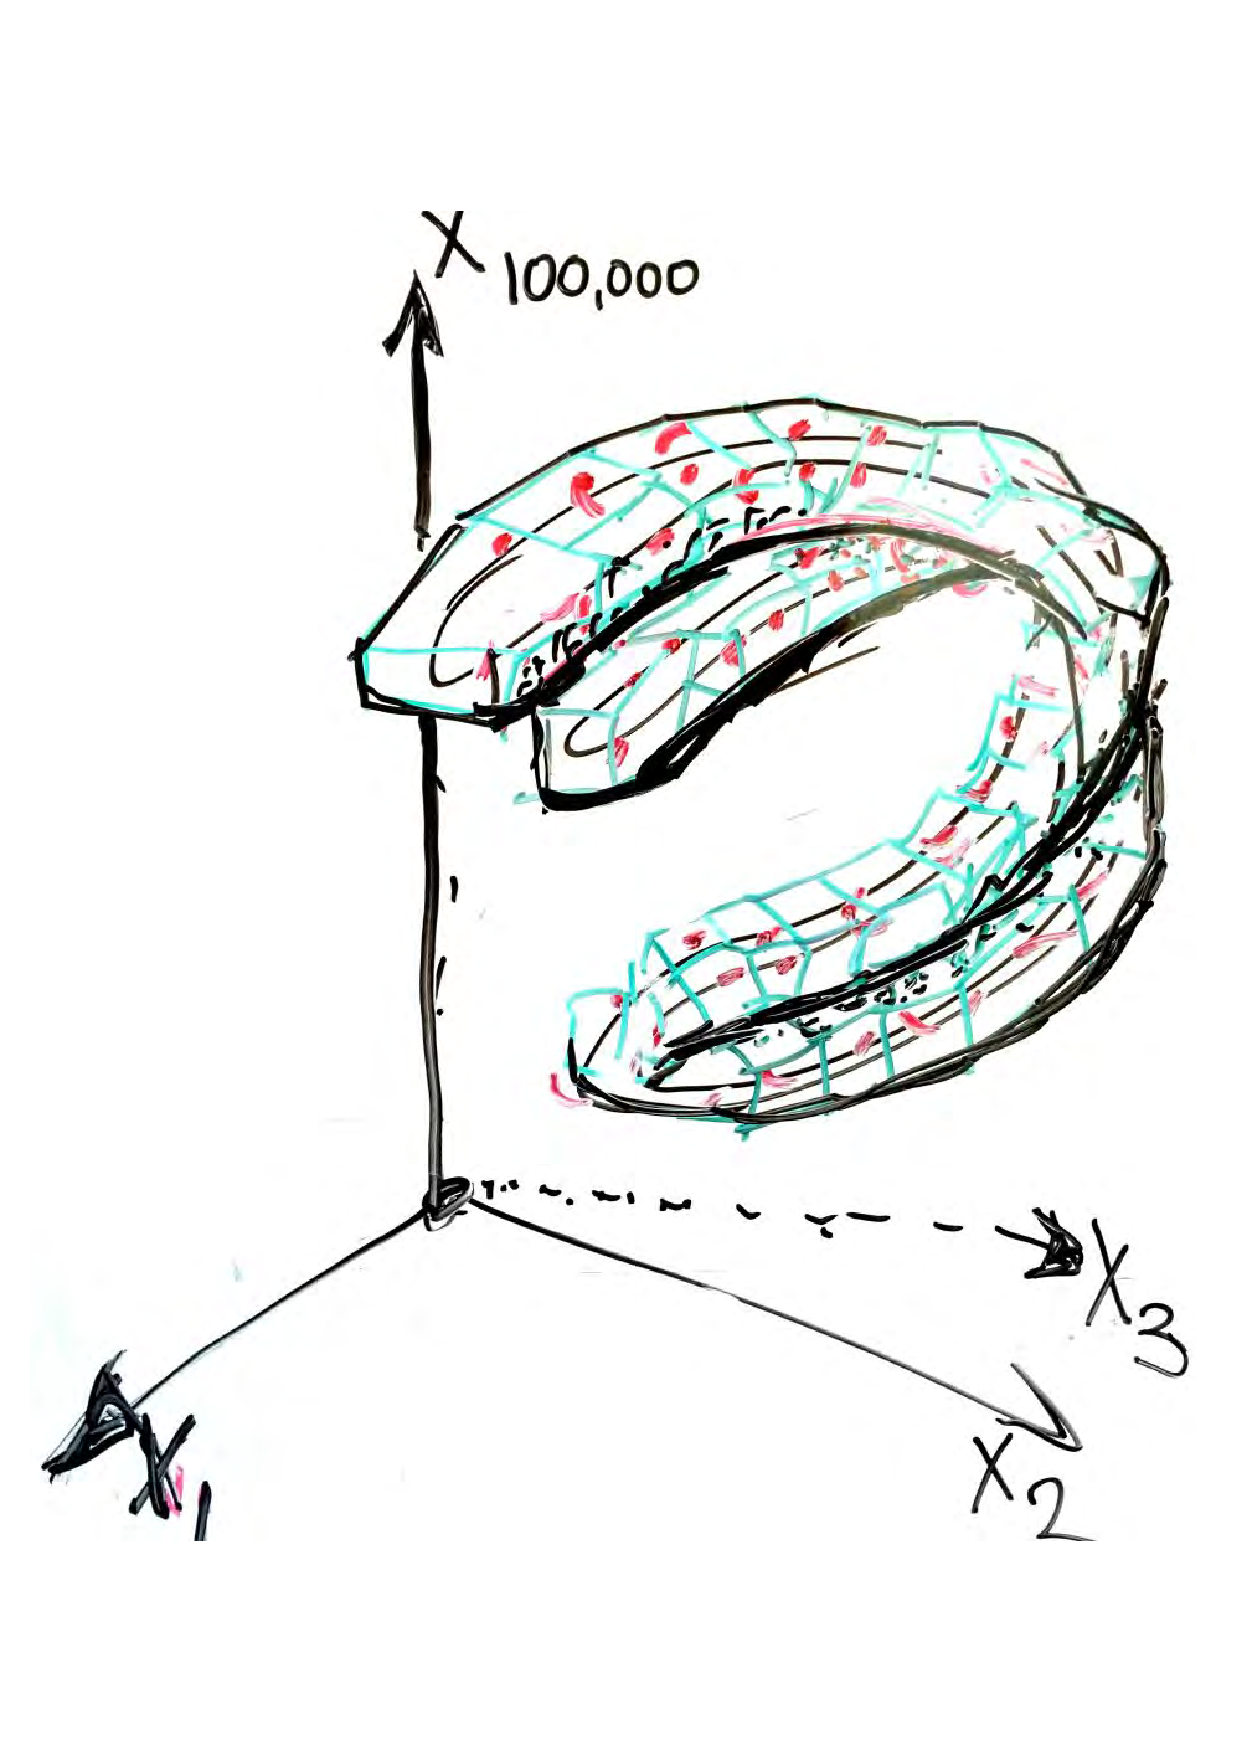
\includegraphics[width=1.00\textwidth]{inertialMan}
\end{center}
    \end{minipage}

\medskip
strange attractor stuffed into
a \textcolor{red}{\Large finite-dimensional} body bag
\end{frame}

\begin{frame}{}
\begin{enumerate}
              \item {\Large
why are we here
                  }\textcolor{gray}{\small
              \item
\statesp
             \item
dimension of the inertial manifold
                    }
            \end{enumerate}
\end{frame}



\begin{frame}{a life in extreme dimensions}
\begin{block}{Navier-Stokes equations (1822)}
\[
\dfrac{\partial \bv}{\partial t} + (\bv \cdot \nabla) \bv
	\,=\,
\frac{1}{R} \nabla ^2 \bv
-\nabla p
+ \mathbf{f}
    \,,\qquad
\nabla \cdot \bv = 0,
\]
\end{block}

\hfill{\small
velocity field  $\bv \in \mathbb{R}^3$
;
pressure field $p$
;
driving force $\mathbf{f}$
        }

\medskip

\begin{block}{describe turbulence}
starting from the equations
{\color{red} (no statistical assumptions)}
\end{block}

\bigskip

\end{frame}

\begin{frame}{}
\begin{enumerate}
              \item {\Large
why is Cvitanovi\'c talking?
                  }\textcolor{gray}{\small
              \item
\statesp
             \item
dimension of the inertial manifold
                    }
            \end{enumerate}
\end{frame}

\begin{frame}{algorithmic advances}
\bigskip
F. Ginelli, H. Chat\'e, G. Radons, A. Politi,
P. Poggi, A. Turchi, R. M. Samelson,
C. L. Wolfe:
            \begin{block}{computation of covariant ``Lyapunov'' vectors}
\HREF{http://doi.org/10.1103/PhysRevLett.99.130601}{\scriptsize Phys. Rev. Lett. 99, 130601 (2007)};
\HREF{http://doi.org/10.1111/j.1600-0870.2007.00234.x}{\scriptsize Tellus A 59, 355 (2007)};\\
\HREF{http://doi.org/10.1088/1751-8113/46/25/254005}{\scriptsize J. Phys. A 46, 254005 (2013)}
            \end{block}
\begin{block}{
covariant vectors are non-normal
}
\begin{center}
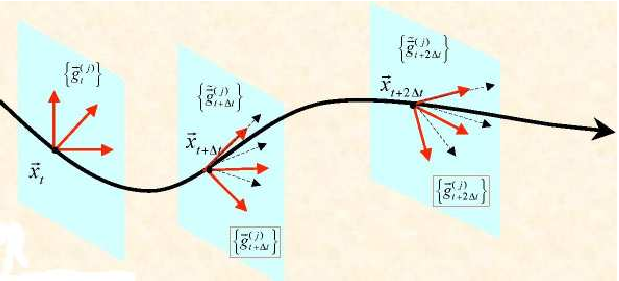
\includegraphics[width=0.7\textwidth]{GinelliFrames}
\end{center}
\end{block}


\vfill\hfill
{\scriptsize \color{yellow} (references are hyperlinked)}
\end{frame}

\begin{frame}{beautiful insights of}
F. Ginelli, H. Chat\'e, G. Radons, A. Politi,
P. Poggi, A. Turchi, H.-l. Yang,
K. A. Takeuchi
% X. Ding, P. Cvitanovi\'c:

\bigskip
{\color{red} physical dynamics} is hyperbolically separated
from \\ the infinity of {\color{red} transient modes} :

            \begin{block}{physical dimension of an inertial manifold}
{\scriptsize
\HREF{http://doi.org/10.1103/PhysRevLett.102.074102}{Phys. Rev. Lett. 102, 074102 (2009)};
\HREF{http://doi.org/10.1103/PhysRevE.84.046214}{Phys. Rev. E 84, 046214 (2011)};\\
\HREF{http://doi.org/10.1103/PhysRevLett.117.024101}{Phys. Rev. Lett. 117, 024101 (2016)}
}
            \end{block}

\bigskip

\begin{itemize}
  \item \KS? OK!
  \item complex Ginzburg-Landau? OK!
  \item \NS? dunno...
\end{itemize}

\vfill\hfill
{\scriptsize \color{yellow} (references are hyperlinked)}
\end{frame}

\begin{frame}{the killer slide}
\KS\ Lyapunov spectrum \\ cells $L=22, 96, 192$ : it scales!
\begin{center}
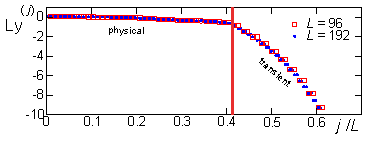
\includegraphics[width=1.0\textwidth]{YaTaGiChRa08fig4a}
\end{center}

Now double \# computational elements, fixed $L$ : \\
all new ones go to the \transient\ spectrum
\footnote{\footnotesize
Yang et al (Phys. Rev. Lett. 2009)}
\end{frame}

\begin{frame}{what this talk is about:}
\begin{block}{
the attracting set of a dissipative flow}
is embedded with the (curvilinear) inertial manifold \\
embedded into $\infty$\dmn\ state space
\begin{center}
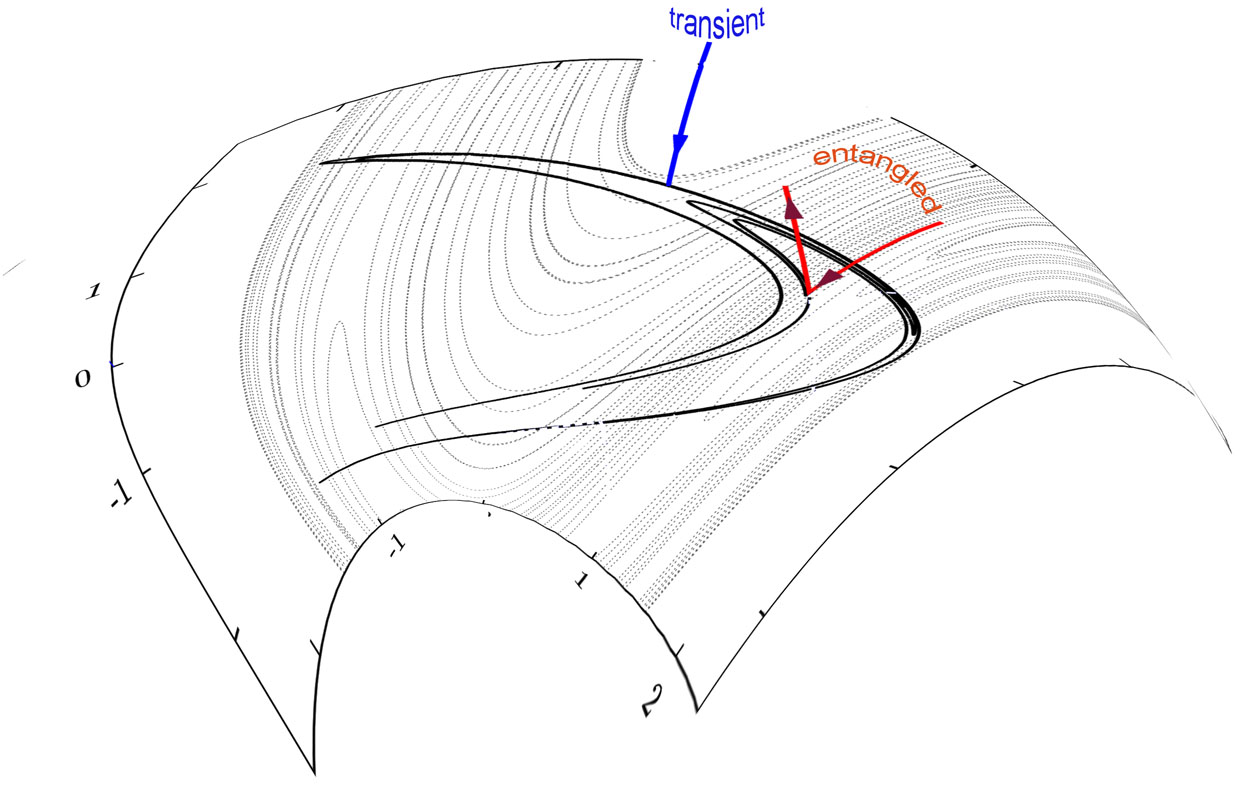
\includegraphics[width=0.7\textwidth]{BoPo10-Fig1c}
\end{center}
\end{block}
but try to draw THAT :)
\end{frame}


\begin{frame}{what this talk is about:}
\begin{block}{
        \only<1>{
it is believed that the attracting set of a dissipative flow
        }
        \only<2>{
\statesp\ of dissipative flow is split into
        }
        \only<3>{
inertial manifold
        }
        \only<4>{
goal : construct \textbf{inertial manifold} for a turbulent flow
        }
}
\begin{center}
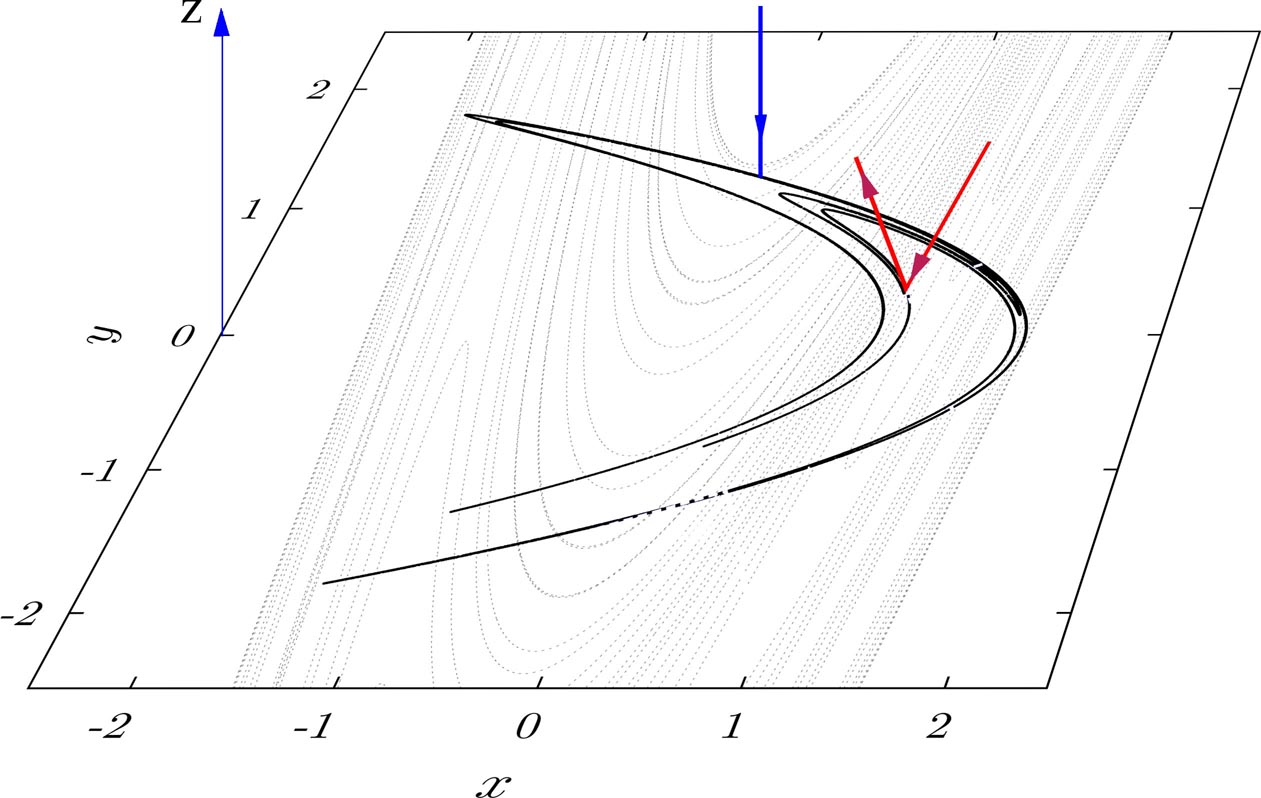
\includegraphics[width=0.7\textwidth]{BoPo10-Fig1b}
\end{center}
\end{block}
\begin{itemize}
        \only<1>{

  \item is confined to  : \\
a finite-dimensional smooth
\textcolor{red}{\emph{inertial manifold}}
  \item ``$z$'' directions : \\
the remaining
$\infty$ of \textcolor{blue}{\em \transient\ dimensions}
        }
        \only<2>{
  \item inertial manifold :
spanned locally by
\textcolor{red}{\entangled\ \cLvs}, tangent to unstable / stable manifolds
  \item the rest : spanned by the remaining
$\infty$ of the contracting, decoupled,
\textcolor{blue}{\transient\ \cLvs}
        }
        \only<3>{
  \item
dynamics of the \textcolor{red}{vectors} that span the inertial manifold is \entangled,
with small angles and frequent tangencies
  \item
a \textcolor{blue}{\transient\ \cLv} : isolated, \\
nearly orthogonal to all other \cLvs
        }
        \only<4>{
  \item
tile it with a finite collection of bricks centered on \\
recurrent states,
each {\textcolor{red}{brick $\approx 10-100$ dimensions}}
  \item
span of $\infty$ of \textcolor{blue}{\transient\ \cLvs} : \\
no intersection with the \entangled\ modes
        }
\end{itemize}

\end{frame}


\begin{frame}{if all this works out, it is kinda amazing}
            \begin{block}{computation of turbulent solutions}
requires at least
\\
$\to$ integration of  $10^4$-$10^6$ coupled ordinary differential equations
            \end{block}

\bigskip

\begin{block}{inertial manifold, tiled}
50 linear tiles cover the (nonlinear, curved) inertial manifold

\medskip

each tile 100 dimensional \hfill \textcolor{green}{\small (fingers crossed :)}
            \end{block}
\end{frame}


\begin{frame}{part 1}
\begin{enumerate}
              \item {\Large
why are we here
                  }\textcolor{gray}{\small
              \item
\statesp
             \item
dimension of the inertial manifold
                    }
            \end{enumerate}
\end{frame}


\begin{frame}{pipe experiment data point}
\begin{block}{a state of turbulent pipe flow at instant in time}
\end{block}

\bigskip

%%%%%%%%%%%%%%%%%%%%%%%%%%%%%%%%%%%%%%%%%%%%%%%%%%%%%%%%%%%%%%%%%%
%\hfill
%\begin{minipage}[c]{0.35\textwidth}
Stereoscopic Particle Image Velocimetry $\to$
3-$d$ velocity field over the entire pipe%
\footnote{\footnotesize
%"Stereoscopic PIV on transition in pipe flow",
Casimir W.H. van Doorne
(PhD thesis, Delft  2004)
%; 	{\tt www.ahd.tudelft.nl}
}

\bigskip

\begin{center}
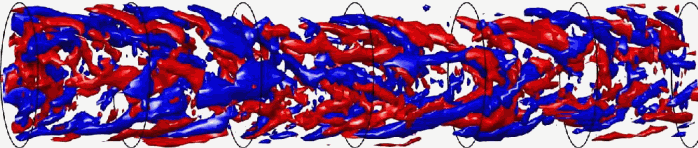
\includegraphics[width=0.90\textwidth]{vDoorne4}
\end{center}
\end{frame}

\begin{frame}{part 2}
\begin{enumerate}
              \item
    \textcolor{gray}{\small
why are we here
        }
              \item
    {\Large
\statesp
    }\textcolor{gray}{\small
              \item
dimension of the inertial manifold
                    }
            \end{enumerate}
\end{frame}


\section[dynamics in $\infty$ dimensions]
{dynamics in $\infty$ dimensions}

\begin{frame}{dynamical description of turbulence}
%	from {../chapter/dynsysII}

\begin{block}{\statesp}
a manifold $\pS \in \reals^{d}$ :
$d$ numbers determine the state of the system
\end{block}

\bigskip

\begin{block}{representative point }
$\ssp(t) \in \pS$
\\
a state of physical system at instant in time
\end{block}

\bigskip

\begin{block}{integrate the equations}
trajectory $\ssp(\zeit) = \flow{\zeit}{\xInit}$ =
representative point time $\zeit$ later
\end{block}
\end{frame}

\begin{frame}{1 spatial dimension ``Navier-Stokes''}

computationally not ready yet to explore \\
the inertial manifold of $3D$ turbulence - we start with

\bigskip

\begin{block}{\KSe}
\[
  u_t + u \triangledown u \,=\,
    {\color{red}-}\triangledown^2 u {\color{red}-\triangledown^4 u}
    \,,\qquad   x \in [-L/2,L/2]
    \,,
\]
\end{block}

\bigskip

describes spatially extended systems such as
\begin{itemize}
 \item flame fronts in combustion
 \item reaction-diffusion systems
 \item \ldots
\end{itemize}

\end{frame}

\section[KSe, $L=22$]{\KS, $L=22$, state space }
\begin{frame}{\KS\ on a large spacetime domain}
\begin{center}
  \includegraphics[width=0.57\textwidth] %,height=0.5\textheight,clip=true]
  {KSL100N256} %{ksevol-fig} %{ks_largeL_cbar}
\end{center}
{\footnotesize
[horizontal] space $\ssp \in [0,100]$ % Xiong's 2017-03-04
\qquad
{[up]} time evolution
}

\begin{itemize}
\item turbulent behavior
\item simpler physical, mathematical and computational setting than Navier-Stokes
\end{itemize}
\end{frame}


\subsection{types of solutions}
\begin{frame}{evolution of \KS\ on small periodic domain}
\begin{center}
  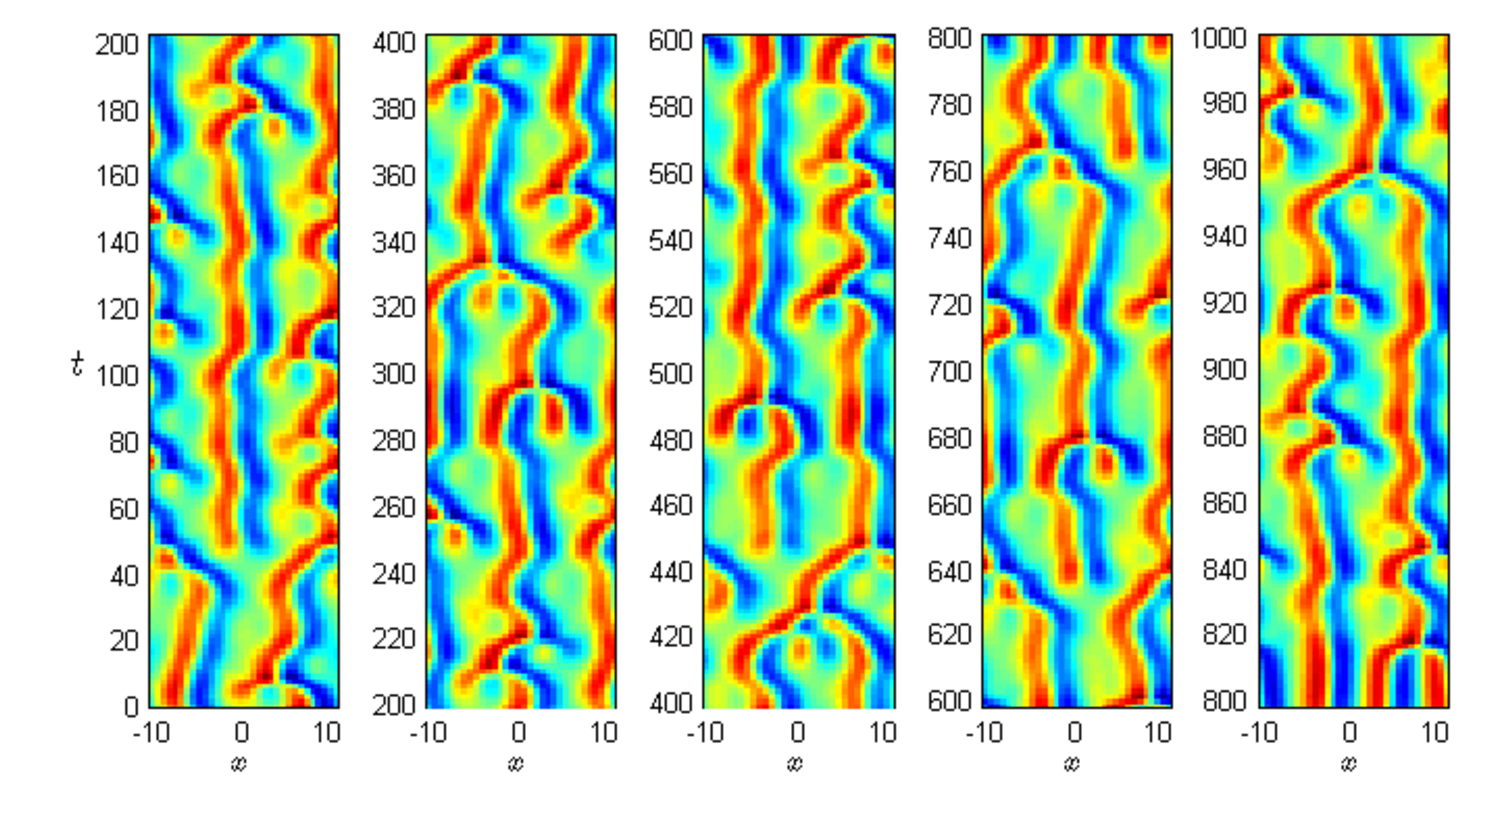
\includegraphics[width=0.9\textwidth,clip=true]{ks_L22_long_orbit}
\end{center}
{\footnotesize
[horizontal] space $\ssp \in [-11,11]$
\qquad
{[up]} time evolution

\medskip

color: magnitude of $u(x,t)$
}
\end{frame}

\begin{frame}{a \rpo}
\begin{block}{full \statesp\ : many periods}
\begin{center}
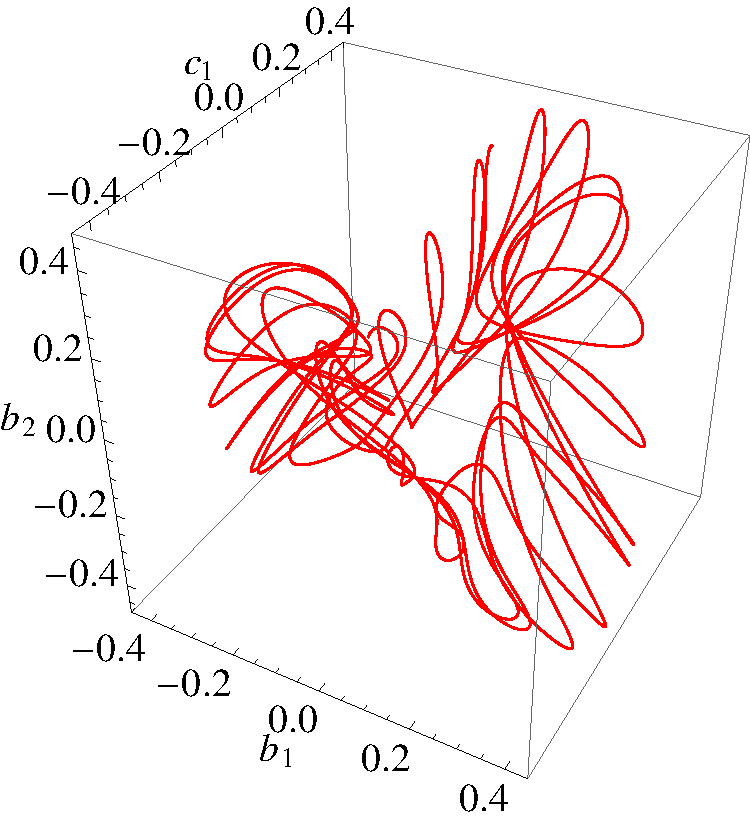
\includegraphics[width=0.5\textwidth]{ks22torRPO1}
\end{center}
\end{block}
have computed: 60\,000 \po s
\end{frame}

\begin{frame}{can explore shadowing}
\begin{center}
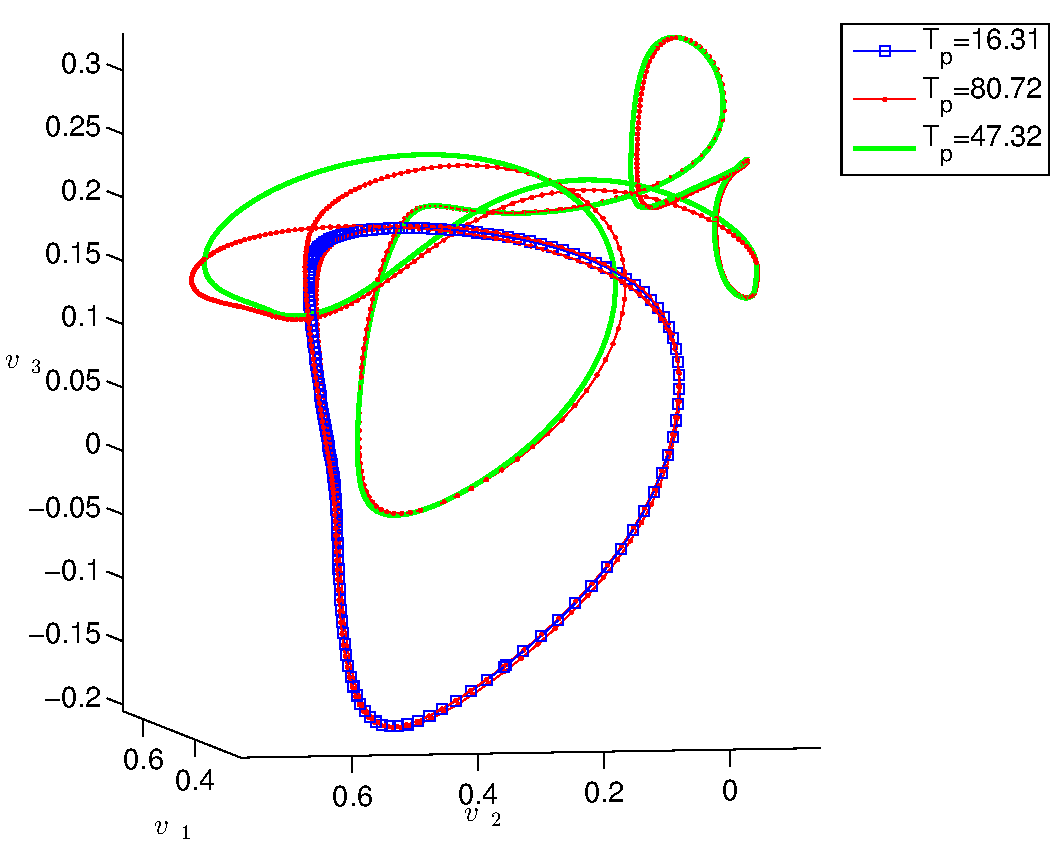
\includegraphics[width=0.6\textwidth]{ks22rpoT8072shad}
\end{center}
\hfill \color{red}{(impossible without symmetry reduction)}
\end{frame}

\begin{frame}{\po s are dense in the attractor}
\begin{center}
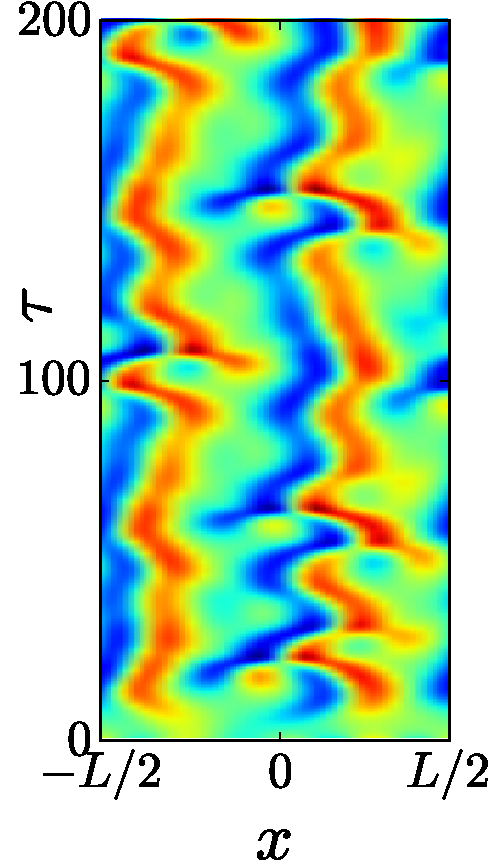
\includegraphics[height=0.52\textwidth]{ksRecycled-ConfErgodic}
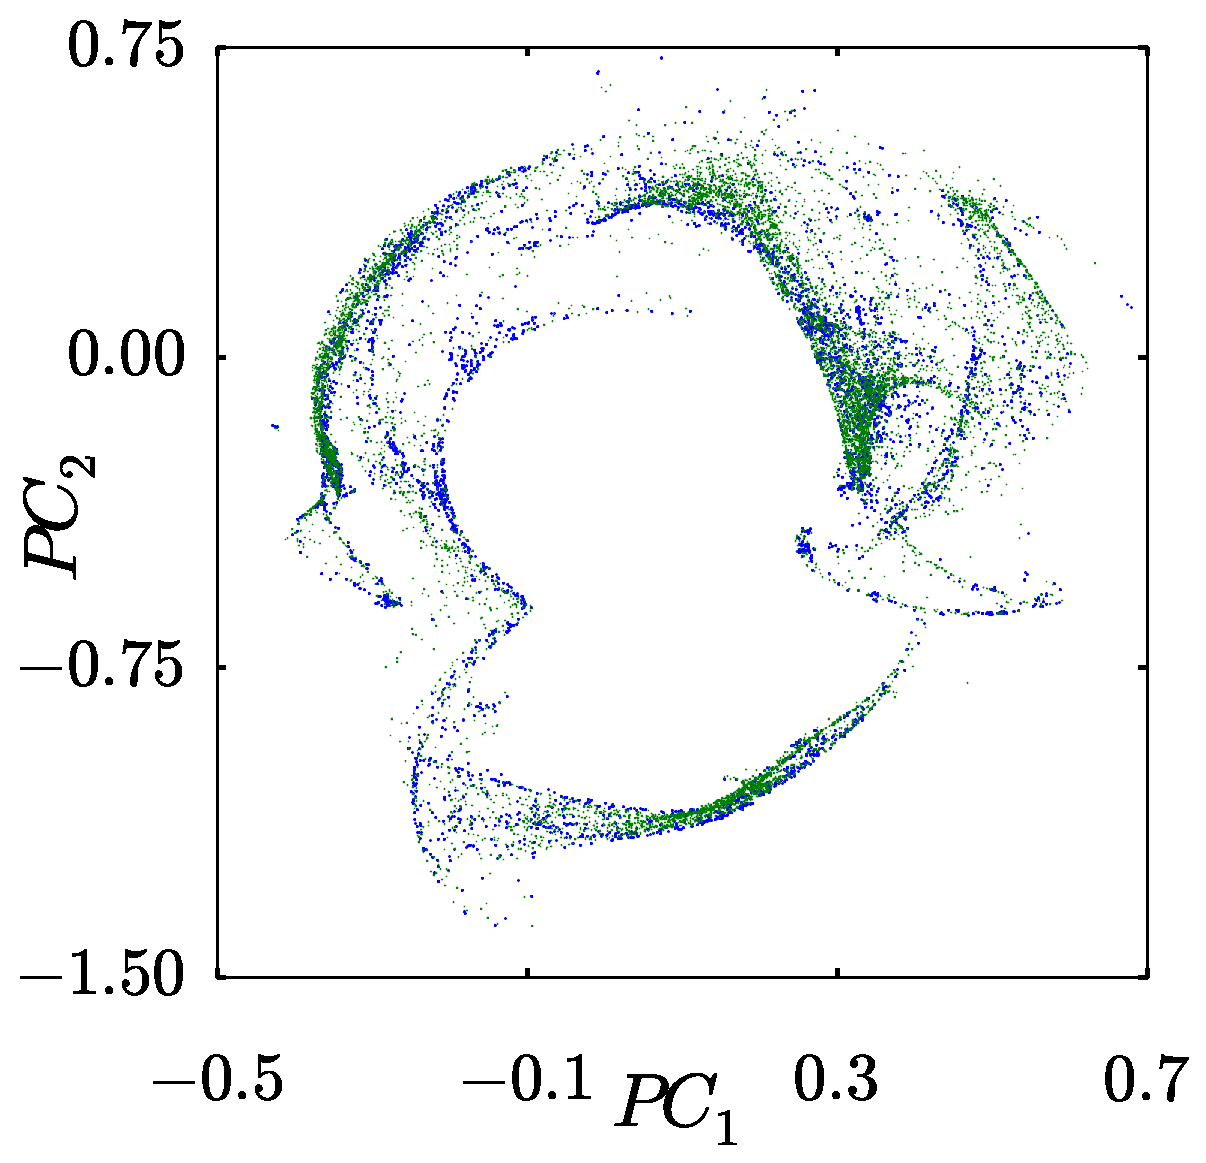
\includegraphics[width=0.545\textwidth]{ksPsectonPCA_POandErgodic}
\end{center}
\begin{itemize}
  \item {[left]} \textcolor{green}{turbulent trajectory} segment in [space$\times$time]
  \item \Poincare\ section, \textcolor{green}{turbulent trajectory} (natural measure)
  \item \textcolor{blue}{periodic points, from $479$ \po s}%
\footnote{\footnotesize
Budanur (PhD thesis 2015)}
\end{itemize}

\end{frame}

\section[dimension of the inertial manifold]
{dimension of the inertial manifold}

\begin{frame}{part 3}
\begin{enumerate}
              \item
    \textcolor{gray}{\small
why are we here
              \item
\statesp
    }
              \item
    {\Large
dimension of the inertial manifold
                    }
            \end{enumerate}
\end{frame}

\begin{frame}{what is the dimension of the inertial manifold?}
we determine it in 6 independent ways

\bigskip

\begin{itemize}
  \item Lyapunov exponents (diagnostic only, previous work)
  \item Lyapunov vectors (sharp, previous work)
  \item four \po s\ determinations (presented here)
\end{itemize}
\end{frame}

\begin{frame}{linearized deterministic flow}

%%%%%%%%%%%%%%%%%%%%%%%%%%%%%%%%%%%%%%%%%%%%%%%%%
 \begin{center}
  \setlength{\unitlength}{0.65\textwidth}
  %% \unitlength = units used in the Picture Environment
  \begin{picture}(1,0.48527529)%
    \put(0,0){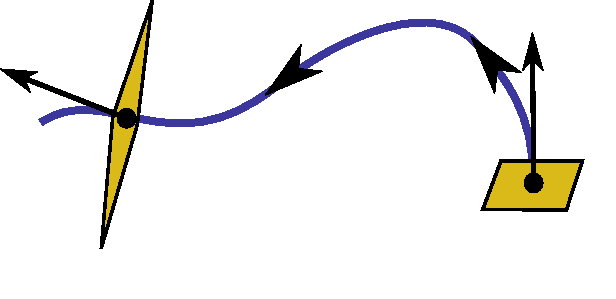
\includegraphics[width=\unitlength]{covariant1}}%
    \put(0.82300289,0.05462827){\color[rgb]{0,0,0}\rotatebox{0.03306771}{\makebox(0,0)[lb]{\smash{$\ssp_n$}}}}%
    \put(0.25001124,0.20377481){\color[rgb]{0,0,0}\rotatebox{0.03306771}{\makebox(0,0)[lb]{\smash{$\ssp_{n+1}$}}}}%
    \put(0.39195273,0.41066662){\color[rgb]{0,0,0}\rotatebox{0.03306771}{\makebox(0,0)[lb]{\smash{$\jMps_n$}}}}%
    \put(0.89193475,0.41023002){\color[rgb]{0,0,0}\rotatebox{0.03306771}{\makebox(0,0)[lb]{\smash{$\vel_n$}}}}%
    \put(0.03306474,0.40112261){\color[rgb]{0,0,0}\rotatebox{0.03306771}{\makebox(0,0)[lb]{\smash{$\vel_{n+1}$}}}}%
  \end{picture}%
 \end{center}
%%%%%%%%%%%%%%%%%%%%%%%%%%%%%%%%%%%%%%%%%%%%%%%%%
\[
\ssp_{n+1} + \orbitDist_{n+1}= f(\ssp_n) + \jMps_n \, \orbitDist_n
      \,, \quad
\jMps_{ij} = \partial f_i / \partial \ssp_j
\]

\medskip

in one time step a linearized neighborhood of $\ssp_n$ is
\begin{enumerate}
	\item[(1)] advected by the flow
	\item[(2)]
transported by the \jacobianM\ $\jMps_n$ into a
neighborhood given by the $\jMps$
eigenvalues and eigenvectors
\end{enumerate}
\end{frame}

\begin{frame}{method (0) : global ergodic trajectory, $t\in[-\infty,\infty]$}
\begin{block}{
Ginelli \etal, Phys. Rev. Lett. (2007)
}
\begin{center}
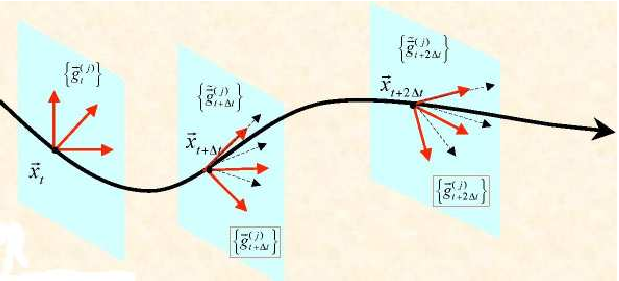
\includegraphics[width=0.7\textwidth]{GinelliFrames}
\end{center}
\end{block}
\JacobianM\ :
orthogonal frame $\to$ non-orthogonal frame
\\
$\to$
\\
QR decomposed into an $R$-matrix + Gram-Schmidt
frame\\
$\to$
\\
 next \jacobianM, and so on
\end{frame}

\begin{frame}{eigenvectors spanning ``physical'' manifold}
\begin{center}
  \setlength{\unitlength}{0.60\textwidth}
  %% \unitlength = units used in the Picture Environment
  \begin{picture}(1,0.70131029)%
    \put(0,0){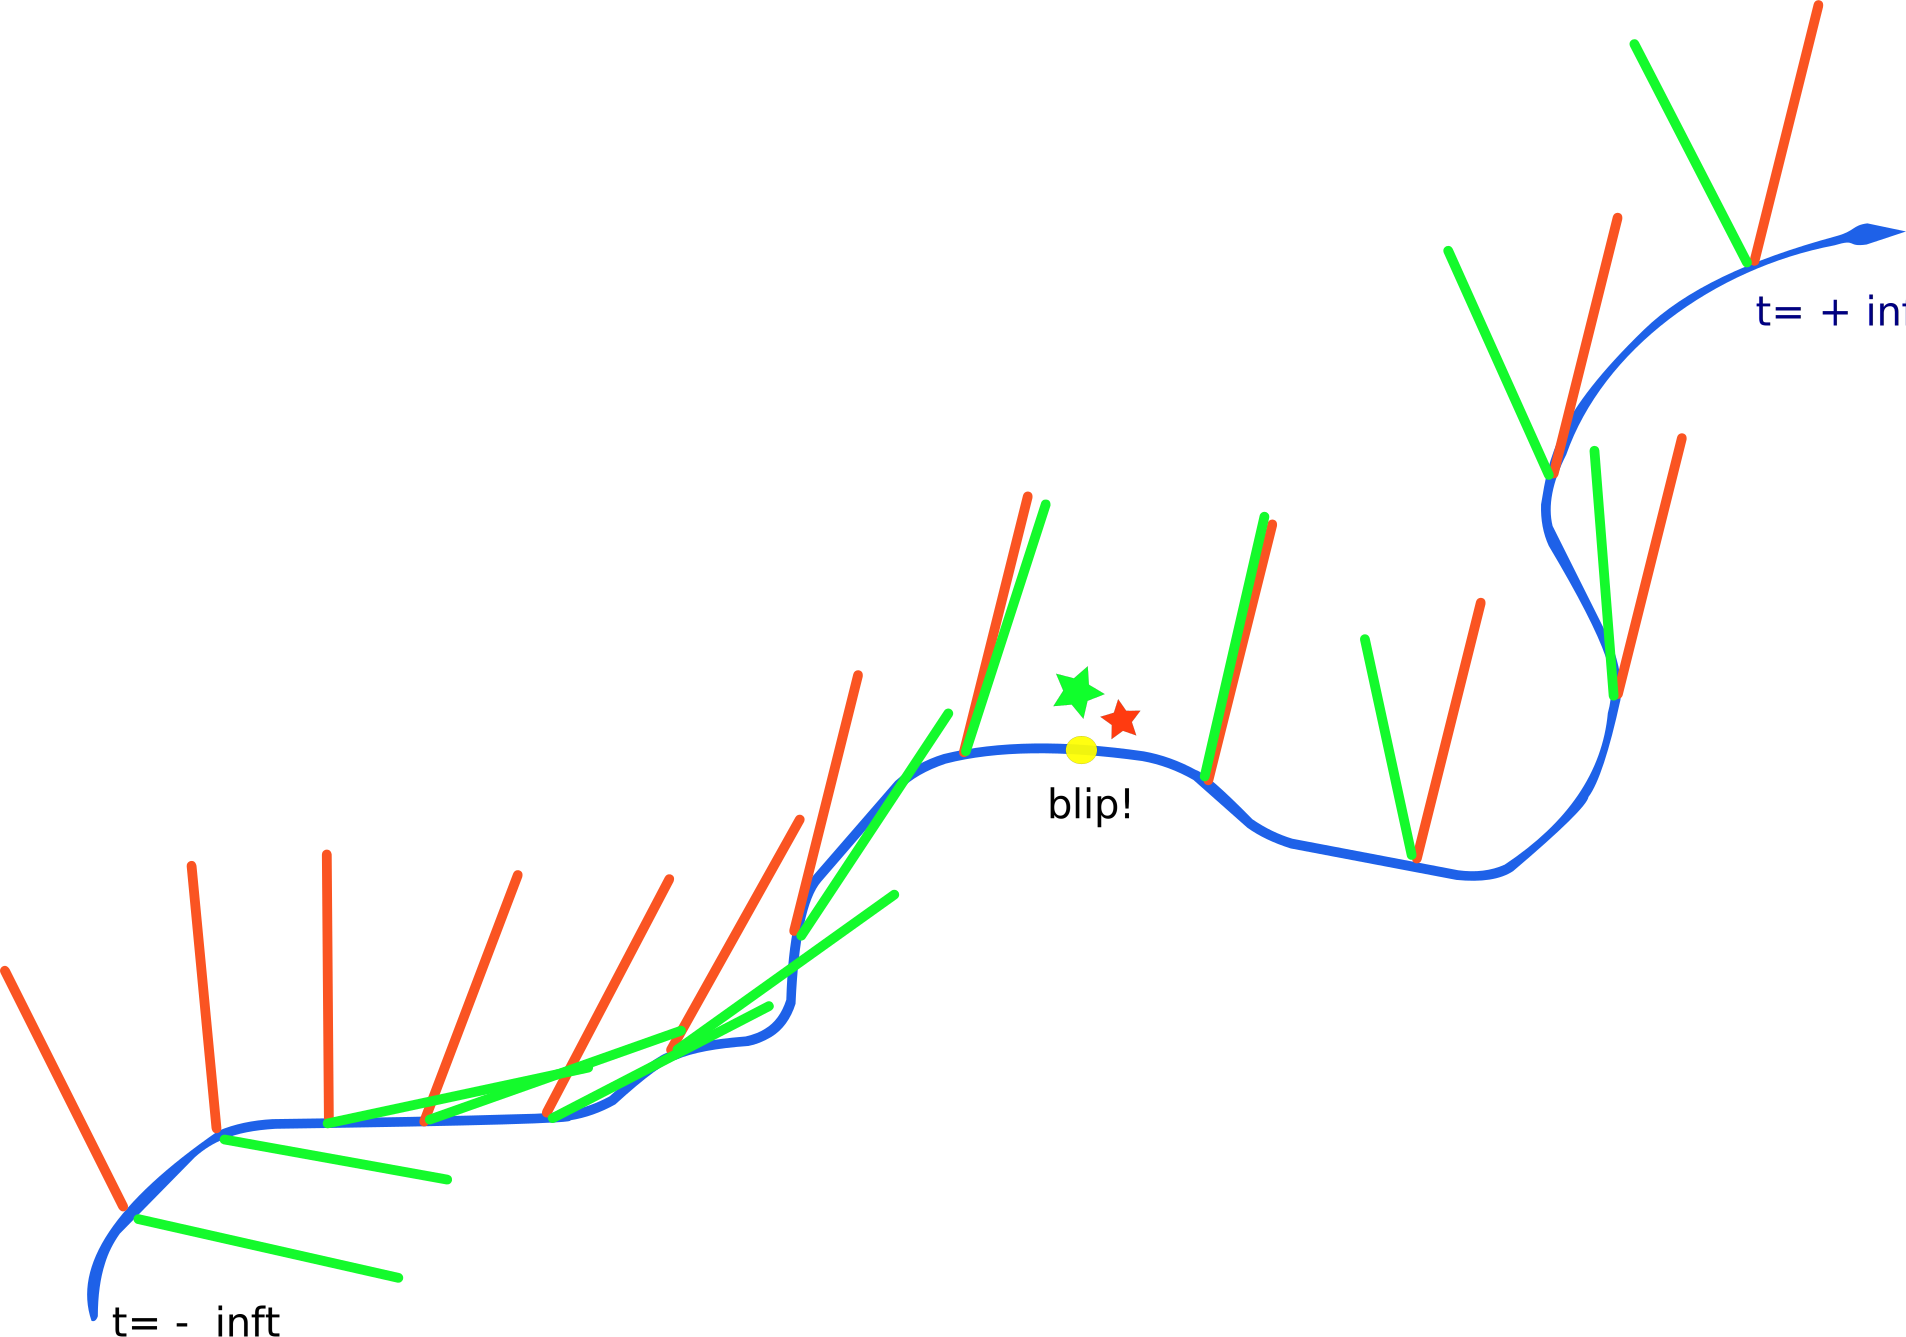
\includegraphics[width=\unitlength]{CovVectors}}%
    \put(0.0586945,0.00014339){\color[rgb]{0,0,0}\makebox(0,0)[lb]{\smash{$t= - \infty$}}}%
    \put(0.92102233,0.52060894){\color[rgb]{0,0,0.50196078}\makebox(0,0)[lb]{\smash{$t= +\infty$}}}%
    \put(0.52032284,0.23204497){\color[rgb]{0,0,0}\makebox(0,0)[lb]{\smash{blip!}}}%
  \end{picture}%
%\caption{\label{fig:CovVectors}
\end{center}
a pair of ``\entangled'' eigenvectors\\
distinct Lyapunov exponents\\
dance along $t$ from $-\infty$ to $-\infty$ orbit
\medskip

at the instant ``blip!'' they are (almost?) collinear
\end{frame}

\begin{frame}{(0) distribution of angles between eigenvectors}
\begin{center}
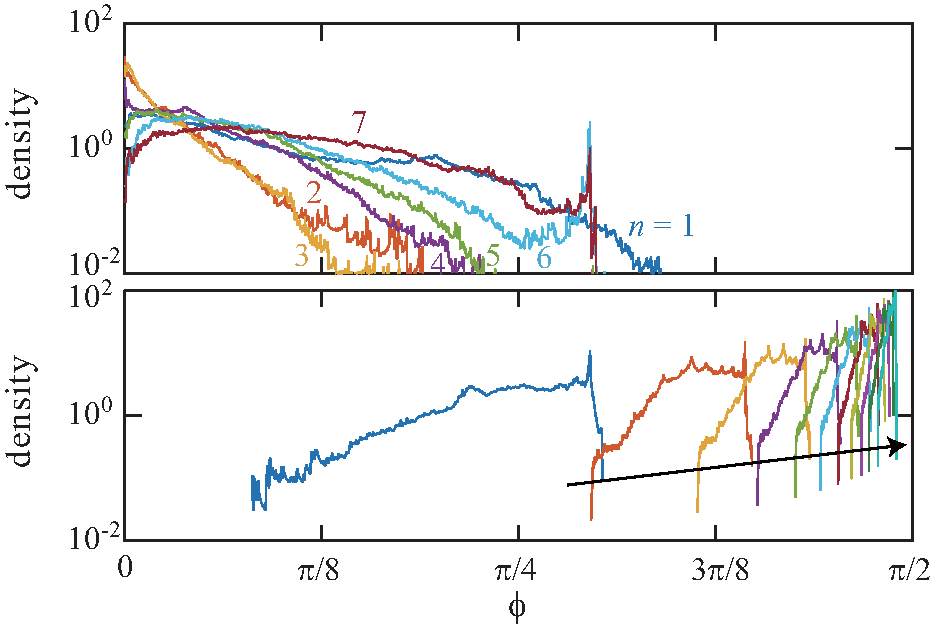
\includegraphics[width=0.6\textwidth]{../../dimension/ks22vecAngles}
\end{center}

histogram of angles between
$n$th leading covariant vector and the next,
accumulated over many long orbits :
\begin{itemize}
  \item
(top) For
$n=1 \cdots 7$ (eigenvector within the \entangled\ manifold) the angles can be
{\color{red}{arbitrarily small}}
  \item
(bottom ) For the remaining, \transient\ eigenvectors,
$n=8,11,12,\cdots$ :
angles are {\color{red}{bounded away from zero}} % Xiong's edit : unity -> zero
\end{itemize}
.\end{frame}

\begin{frame}{}
    \begin{minipage}[b]{0.30\textwidth}
\begin{block}{
OK, so the the frame is
\\
locally flat
}
\end{block}
    \end{minipage}
~~~~~~
    \begin{minipage}[b]{0.60\textwidth}
\begin{center}
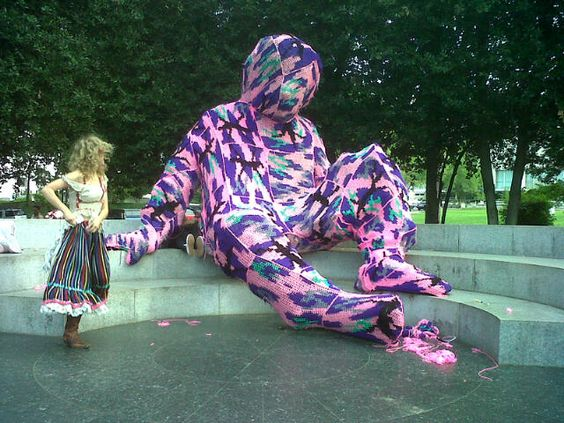
\includegraphics[width=1.00\textwidth]{EinsteinWrapped}
\end{center}
    \end{minipage}

\bigskip\bigskip

\begin{block}{
but where the (blip) are we in the state space?
}
\end{block}


\end{frame}

\begin{frame}{}
    \begin{minipage}[b]{0.30\textwidth}
\begin{block}{
we are
here
}
\end{block}
    \end{minipage}
~~~~~~
    \begin{minipage}[b]{0.50\textwidth}
\begin{center}
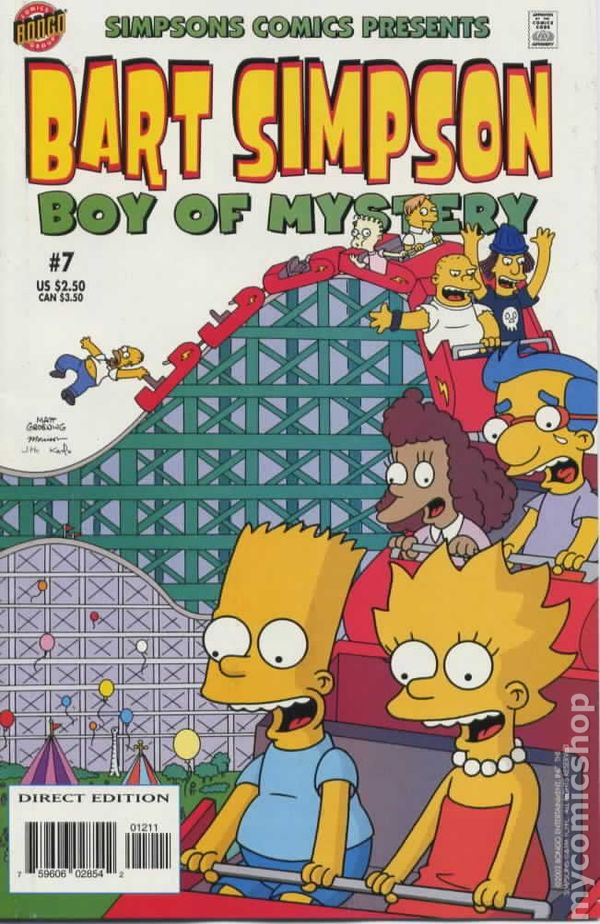
\includegraphics[width=1.00\textwidth]{SimpsonRollerC}
\end{center}
    \end{minipage}

\medskip
next : cartography of a roller coaster ride
\end{frame}


\begin{frame}{part 4}
\begin{enumerate}
              \item
    \textcolor{gray}{\small
why are we here
              \item
\statesp
              \item
dimension of the inertial manifold
    }
              \item
    {\Large
{\color{red} new :} cartography of the inertial manifold
                    }
            \end{enumerate}
\end{frame}


\begin{frame}{cartography for fluid dynamicists}
\bigskip

\textcolor{blue}{cover the inertial manifold with a set of flat charts}

\hfill
\vfill
we can do this with

\hfill \color{red}{finite\dmn\ bricks embedded in $10^{100\,000}$ dimensions}!
\end{frame}

\begin{frame}{tile the inertial manifold by {\Large recurrent flows}}
    \begin{minipage}[b]{0.40\textwidth}
\begin{block}{}
a fixed point

\medskip

a 2-cycle, etc.
\end{block}
    \end{minipage}
~~~~~~
    \begin{minipage}[b]{0.51\textwidth}
\begin{center}
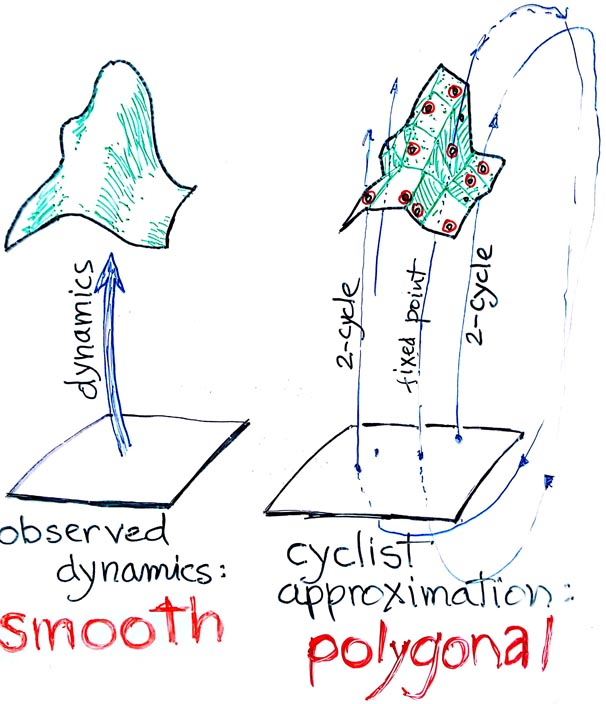
\includegraphics[width=1.00\textwidth]{f_1_08_1}
\end{center}
    \end{minipage}

\medskip

smooth dynamics  (left frame) \\
tesselated by the skeleton of recurrent flows, \\
together with (right frame) their
linearized neighborhoods
\end{frame}


\begin{frame}{charting the inertial manifold}
\begin{center}
  \setlength{\unitlength}{0.60\textwidth}
  %% \unitlength = units used in the Picture Environment
  \begin{picture}(1,0.89907101)%
    \put(0,0){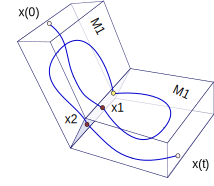
\includegraphics[width=\unitlength]{A29-1ridge}}%
    \put(0.00894598,0.81885604){\color[rgb]{0,0,0}\makebox(0,0)[lb]{\smash{$\sspRed(0)$}}}%
    \put(0.88743345,0.05105926){\color[rgb]{0,0,0}\makebox(0,0)[lb]{\smash{$\sspRed(\zeit)$}}}%
    \put(0.78614059,0.43443027){\color[rgb]{0,0,0}\rotatebox{-25.76142111}{\makebox(0,0)[lb]{\smash{$\pSRed{}^{(2)}$}}}}%
    \put(0.37048948,0.79485578){\color[rgb]{0,0,0}\rotatebox{-61.41291822}{\makebox(0,0)[lb]{\smash{$\pSRed{}^{(1)}$}}}}%
    \put(0.2429401,0.27697318){\color[rgb]{0,0,0}\makebox(0,0)[lb]{\smash{$\sspRed_2$}}}%
    \put(0.47832196,0.33514069){\color[rgb]{0,0,0}\makebox(0,0)[lb]{\smash{$\sspRed_1$}}}%
  \end{picture}%
%\caption{\label{fig:A29-1ridge}
\end{center}
two tangent ``\entangled'' tiles = finite\dmn\ bricks
\medskip

shaded plane : \\
when integrating your equations, switch the local chart
\end{frame}


\begin{frame}{method (1) : local \rpo, one period}
\begin{block}{Ding \& Cvitanovi{\'c}, SIAM J. Appl. Dyn. Syst. (2016)}
\begin{center}
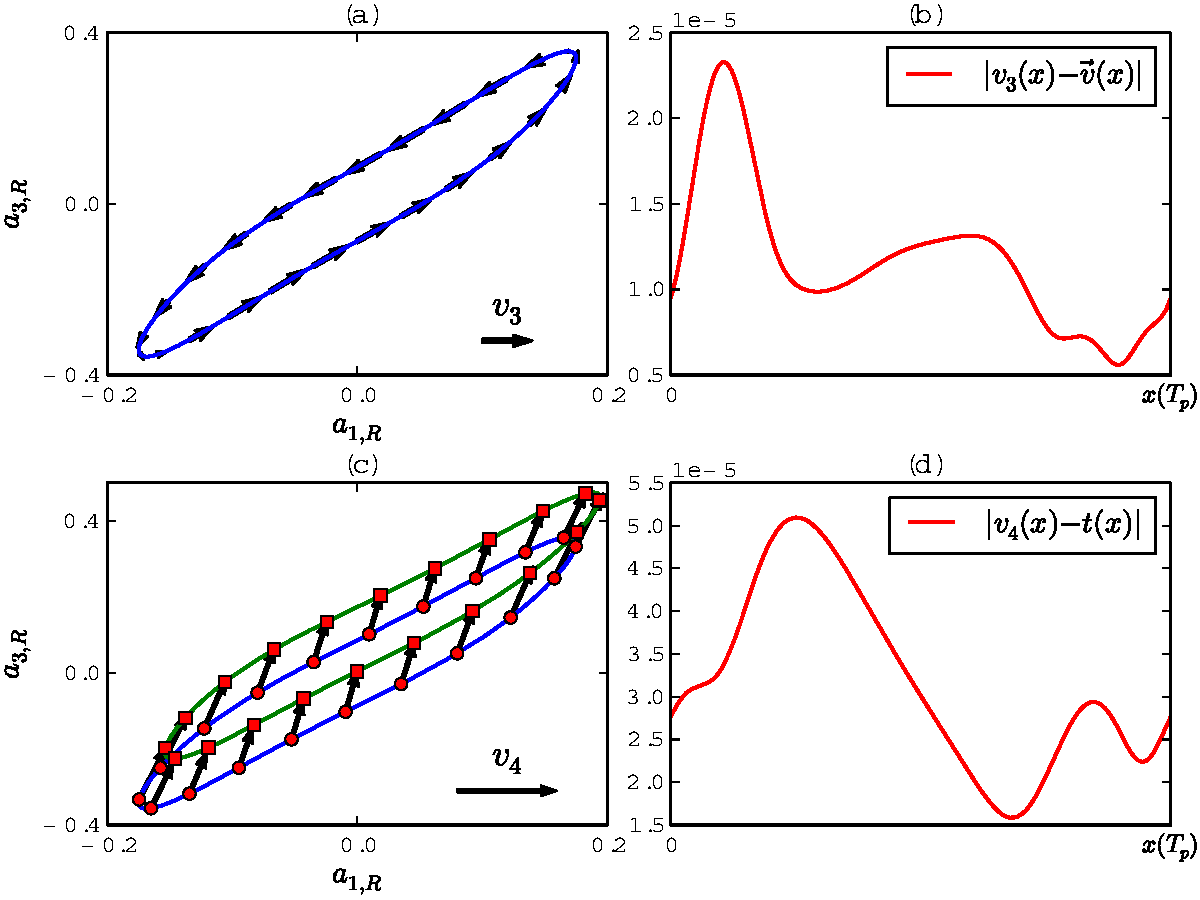
\includegraphics[width=1.0\textwidth]{../../xiong/figures/ppo1vectfield}
\end{center}
\end{block}
[right panel] \\
all eigenvectors computed close to the machine precision
\end{frame}

\begin{frame}{(1) algorithmic breakthrough : \\
            all Floquet exponents to machine precision}
\begin{center}
\small
\begin{tabular}{  c | c | c| } %\label{tab:floquet_exponents_ppo1}

	&  \large{$\eigRe[i]$ }  &\large{$e^{iT_{p}\eigIm[i]}$}   \\
  1=2  & 0.0331970261043278   & -0.42330856002164    \\
	& 			  & + i\,0.905985575499084 \\
  3=4  & (2 marginal) &                          \\
	5  & -0.216338085869672   & 1                         \\
  6=7  & -0.265233812289065   & -0.867175421594352   \\
	& 			  & + i\,0.49800279937231   \\
	\dots & \dots  & \dots                   \\
	29 & -316.19797864063     & 1                         \\
	30 & -320.666664811713    & -1                        \\
	\end{tabular}
	\end{center}
\bigskip

Floquet exponents for the shortest \ppo\ :

\bigskip

$\eigRe[i]$ = real part of the exponent.
\\
either
the multiplier sign for a real exponent, or
\\
$\eigIm[i] \to $
the multiplier phase for a complex Floquet exponent
\end{frame}

\begin{frame}{(1) algorithmic breakthrough : \\
            all Floquet exponents to machine precision}

why is this a big deal?
\bigskip

periodic Schur decomposition : resolves
Floquet multipliers differing by thousands of orders {of magnitude}

\medskip

here the smallest Floquet multiplier
for the shortest \po\ is
\begin{block}{}
\begin{center}
$|\ExpaEig_{62}| \simeq e^{-6080.4\times 10.25} \approx 10^{-27069}$
\end{center}
\end{block}
\end{frame}


\begin{frame}{(1) Floquet and Lyapunov exponents, $L=22$ small cell}
\begin{center}
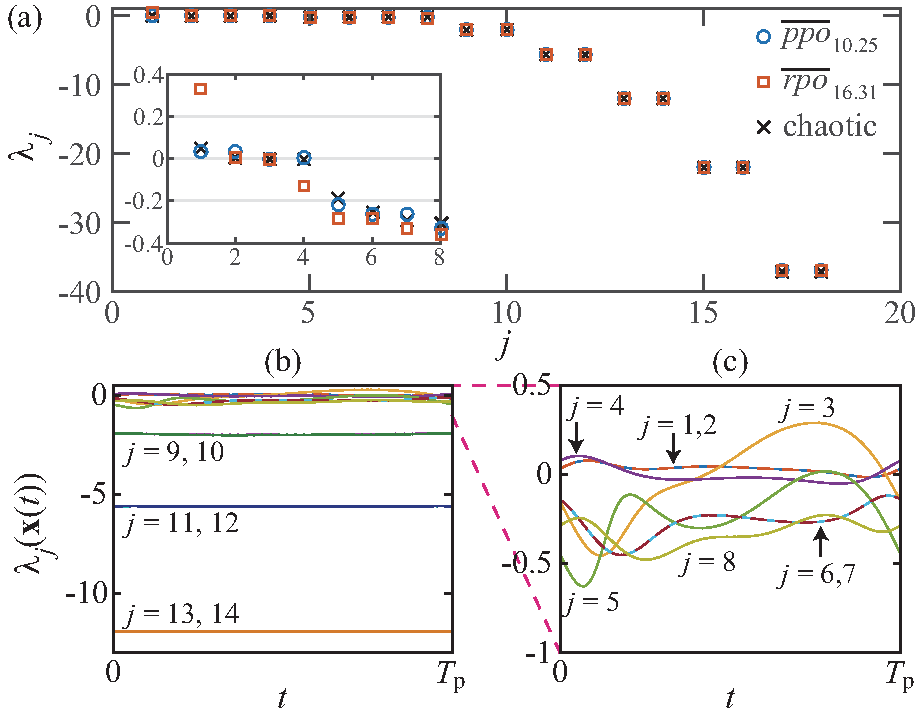
\includegraphics[width=0.85\textwidth]{../../dimension/ks22FloqExp}
\end{center}
8 \entangled\ modes, rest \transient\  :

\hfill \color{red}{inertial manifold is 8 dimensional!}
\end{frame}

\begin{frame}{(1) dimension of the inertial manifold from an individual orbit (??)}
\begin{block}{
   Floquet exponents separate into \entangled\ vs. \transient}
for every single \po! (checked 500 orbits)
\end{block}

\bigskip\bigskip

if true for \NS, that would make life easy!
\end{frame}


\begin{frame}{(2) dimension of the inertial manifold from ensemble of orbits}

\bigskip

\begin{itemize}
  \item principal angles between hyperplanes spanned by Floquet vectors
\end{itemize}
\end{frame}

\begin{frame}{(2) Floquet vectors}
\setlength{\unitlength}{0.40\textwidth}
\begin{center}
              \begin{minipage}[b]{0.40\textwidth}
  \begin{picture}(1,0.66867674)%
    \put(0,0){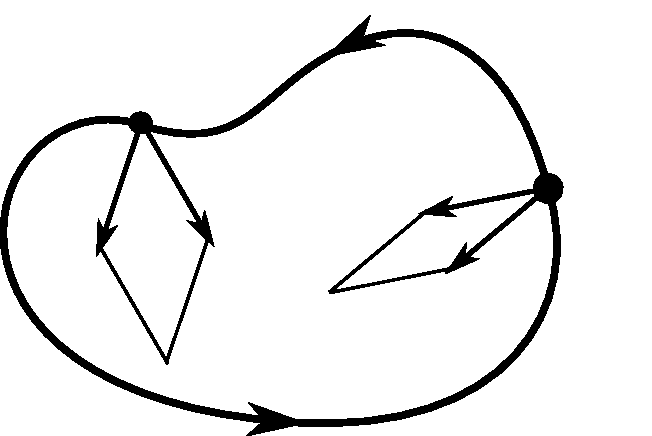
\includegraphics[width=\unitlength]{covariantPO}}%
    \put(0.74435424,0.20540854){\color[rgb]{0,0,0}\rotatebox{0.0313674}{\makebox(0,0)[lb]{\smash{$\jEigvec[1]$}}}}%
    \put(0.64622163,0.40053847){\color[rgb]{0,0,0}\rotatebox{0.0313674}{\makebox(0,0)[lb]{\smash{$\jEigvec[2]$}}}}%
    \put(0.89791873,0.38658395){\color[rgb]{0,0,0}\rotatebox{0.0313674}{\makebox(0,0)[lb]{\smash{$\ssp(0)$}}}}%
    \put(0.12764619,0.54392048){\color[rgb]{0,0,0}\rotatebox{0.0313674}{\makebox(0,0)[lb]{\smash{$\ssp(\tau)$}}}}%
    \put(0.4259836,0.61739585){\color[rgb]{0,0,0}\rotatebox{0.0313674}{\makebox(0,0)[lb]{\smash{$\jMps^\tau$}}}}%
    \put(0.35028678,0.33942992){\color[rgb]{0,0,0}\rotatebox{0.0313674}{\makebox(0,0)[lb]{\smash{$\jEigvec[1]$}}}}%
    \put(0.05904285,0.32095124){\color[rgb]{0,0,0}\rotatebox{0.0313674}{\makebox(0,0)[lb]{\smash{$\jEigvec[2]$}}}}%
  \end{picture}% % \label{f:covariantPO}
              \end{minipage}
\end{center}

\bigskip

a parallelepiped spanned by a pair of Floquet eigenvectors (`covariant
vectors') transported along the orbit

\bigskip

\begin{itemize}
 \item \jacobianM\ not self-adjoint :
the eigenvectors are not orthogonal, the eigenframe is `non-normal'
  \item Measure the angle between eigenvectors \\
$\jEigvec[i](\ssp(\zeit))$ and $\jEigvec[j](\ssp(\zeit))$
\end{itemize}
\end{frame}

\begin{frame}{(2) example : \KS\ \rpo}
\begin{center}
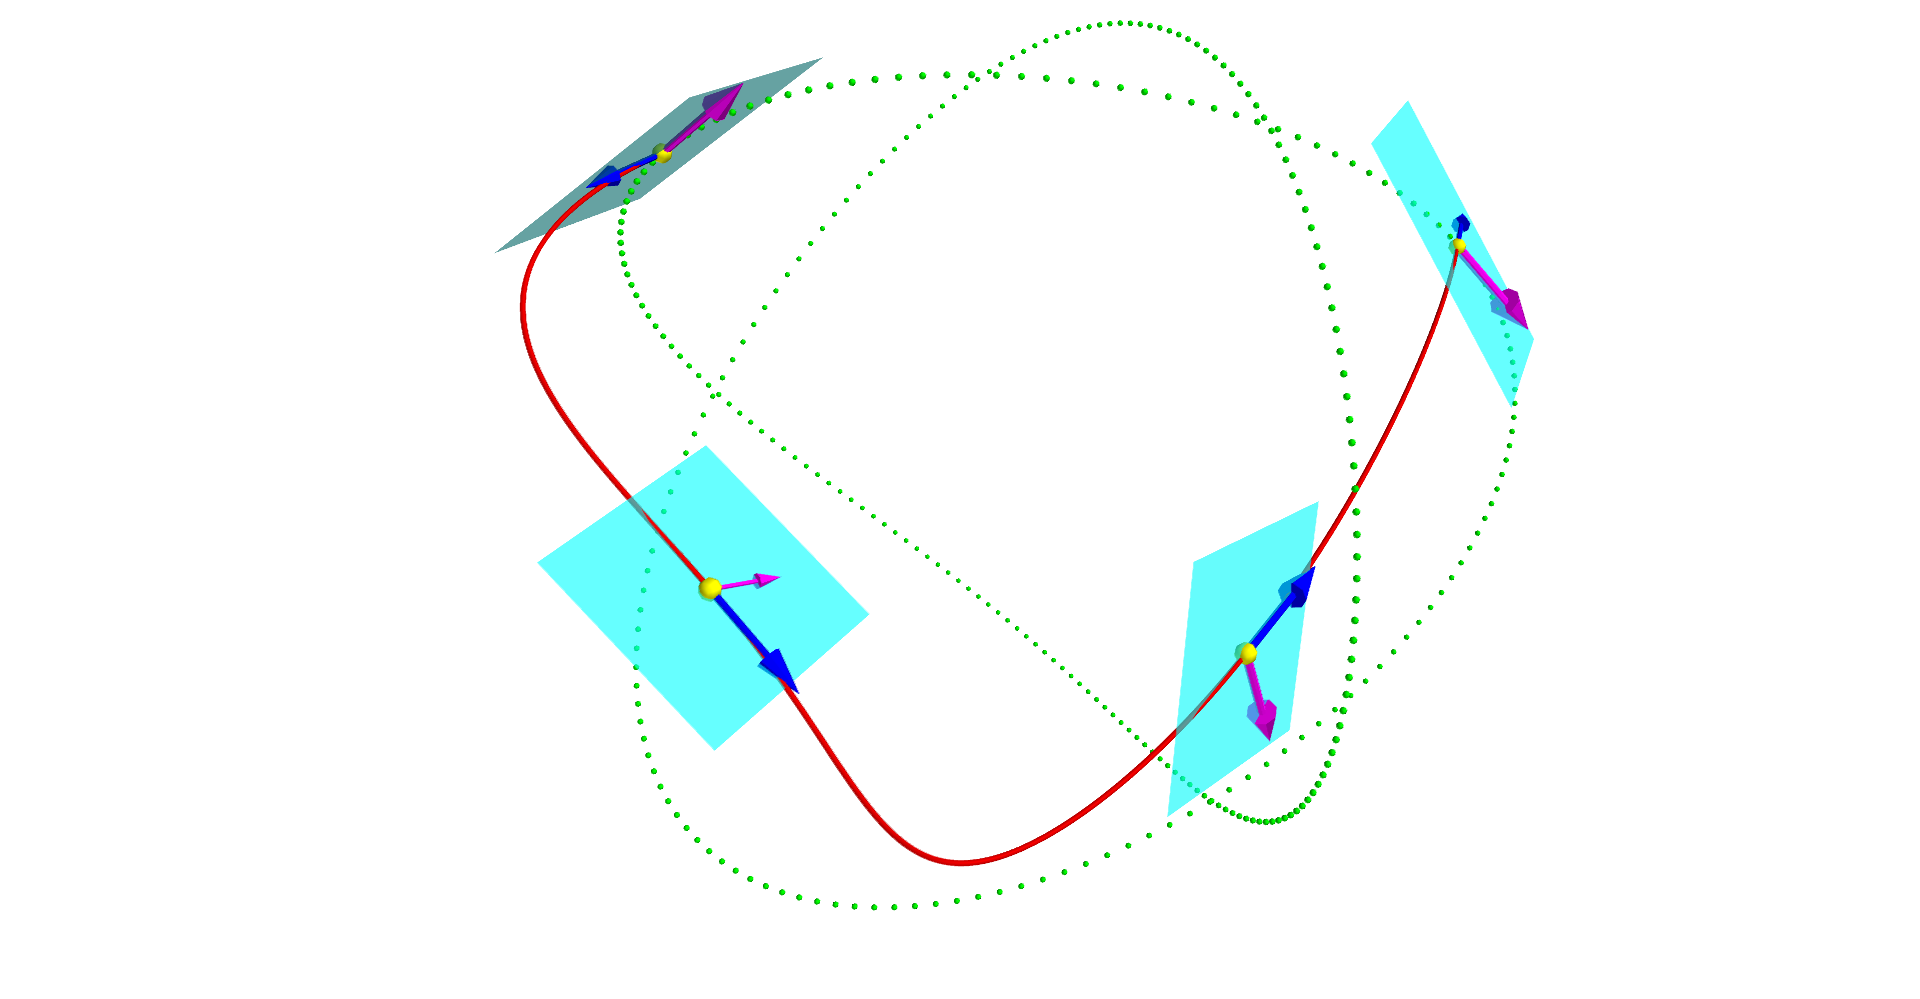
\includegraphics[width=0.9\textwidth]{../../xiong/figures/rpo1_marginal}
\end{center}
dotted green : a group orbit \\
solid red : a \rpo \\
planes : a tangent space spanned and transported by 2 Floquet vectors
\end{frame}

\begin{frame}{(2) distribution of principal angles between Floquet subspaces}
\begin{center}
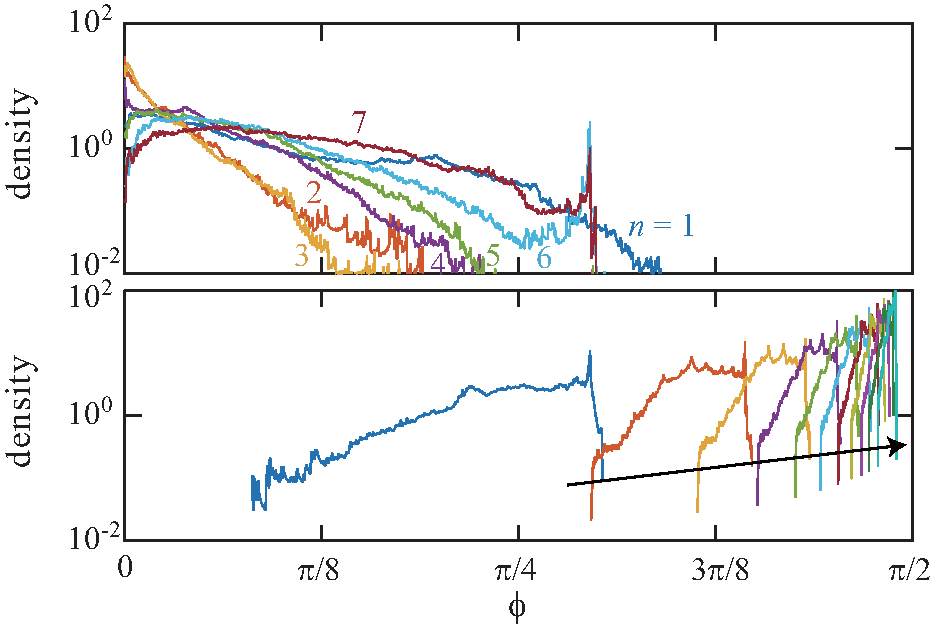
\includegraphics[width=0.6\textwidth]{../../dimension/ks22vecAngles}
\end{center}


histogram of angles between $S_n$
($n$ leading Floquet vectors) and $\bar{S}_n$
(the rest),
accumulated over the 400 orbits :
\begin{itemize}
  \item
(top) For
$n=1 \cdots 7$ ($S_n$ within the \entangled\ manifold) the angles can be
{\color{red}{arbitrarily small}}
  \item
(bottom ) For the $\bar{S}_n$ spanned by \transient\
modes,
$n=8,10,12,\cdots,28$ :
angles {\color{red}{bounded away from unity}}
\end{itemize}
.
\end{frame}

\begin{frame}{(3), (4) dimension of the inertial manifold from \\
        a chaotic trajectory shadowing a given orbit}

\bigskip

two independent measurements

\begin{itemize}
  \item[(3)] shadowing separation vector lies within the orbit's Floquet \entangled\ manifold
  \item[(4)]  shadowing separation vector lies within the chaotic trajectories \cLvs' \entangled\ manifold
\end{itemize}

\bigskip

`separation vector' = difference vector between the chaotic orbit point and
\po\ point at their (locally) closest passage

\medskip

accumulate 1000's of near recurrences


\end{frame}

\begin{frame}{}
    \begin{minipage}[b]{0.35\textwidth}
\begin{block}{(3)}
chaotic trajectory shadows \\
\po s
\\within the
\\
entangled subspace
\end{block}
    \end{minipage}
~
    \begin{minipage}[b]{0.61\textwidth}
\begin{center}
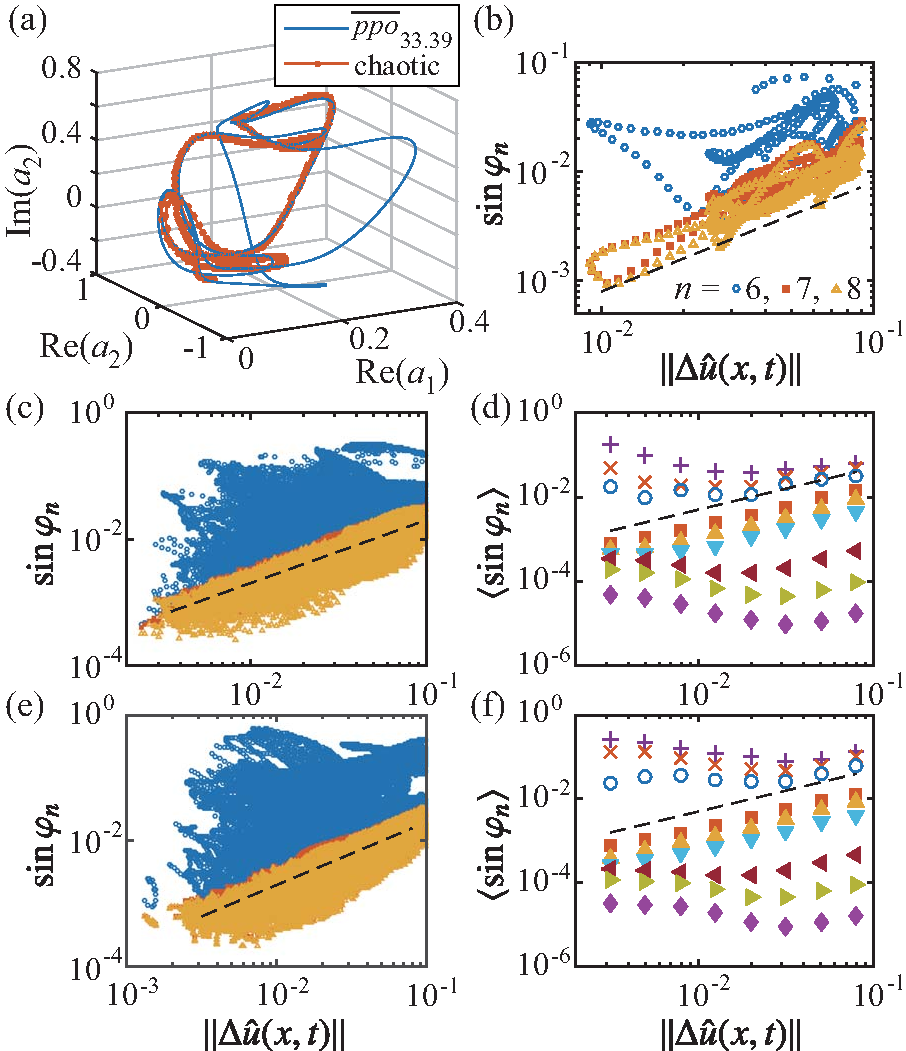
\includegraphics[width=1.00\textwidth]{../../dimension/ks22vecShadow}
\end{center}
    \end{minipage}
\end{frame}


\begin{frame}{what about large or $\infty$ domains ?}
\begin{block}{spatiotemporal chaos}
\begin{center}
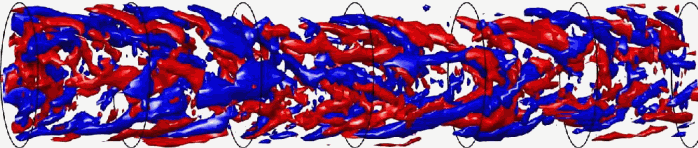
\includegraphics[width=0.90\textwidth]{vDoorne4}
\end{center}
\end{block}

\bigskip

\begin{block}{spatiotemporal chaos is extensive}
\begin{center}
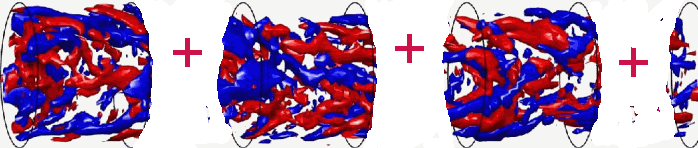
\includegraphics[width=0.90\textwidth]{vDoorne4ext}
\end{center}
\end{block}

\end{frame}


\begin{frame}{\KS\ physical dimension \\
grows linearly with the domain size!}
\begin{center}
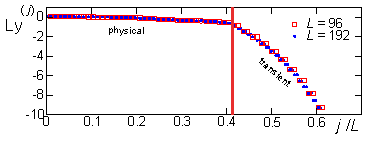
\includegraphics[width=1.0\textwidth]{YaTaGiChRa08fig4a}
\end{center}

Now double \# Fourier modes : all new ones go to the \transient\ spectrum
\footnote{\footnotesize
Yang et al (Phys. Rev. Lett. 2009)}
\end{frame}


\begin{frame}{summary for the impatient}
\begin{block}{\statesp\ of dissipative flow is split into}
\begin{center}
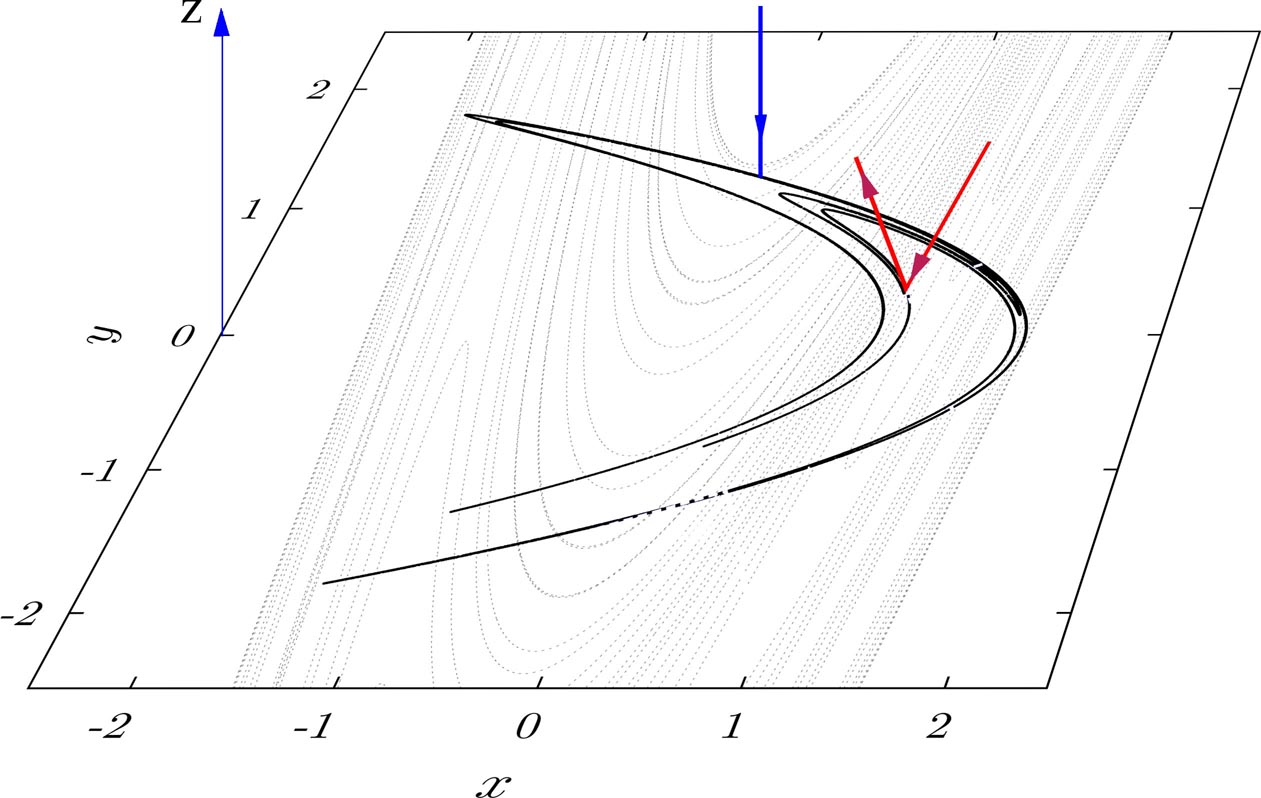
\includegraphics[width=0.7\textwidth]{BoPo10-Fig1b}
\end{center}
\end{block}
\begin{itemize}
  \item inertial manifold :
spanned locally by
\textcolor{red}{\entangled\ \cLvs}, tangent to unstable / stable manifolds
  \item the rest : spanned by the remaining
$\infty$ of the contracting, decoupled,
\textcolor{blue}{\transient\ \cLvs}
\end{itemize}
\end{frame}

\begin{frame}{detailed summary \\
 6 ways to determine the dimension of the inertial manifold}
Tangent spaces separate into \entangled\ vs. \transient

\begin{enumerate}
  \item Lyapunov exponents (plausible, previous work)
  \item Lyapunov vectors (sharp, previous work)
  \item
for each individual orbit Floquet exponents separate into \entangled\ vs.
\transient\ (new)
  \item
for an ensemble of orbits principal angles between hyperplanes spanned by
Floquet vectors separate into \entangled\ vs. \transient\   (new)
  \item
for a chaotic trajectory shadowing a given orbit the separation
vector lies within the orbit's Floquet \entangled\ manifold (new)
  \item
for a chaotic trajectory shadowing a given orbit the separation
vector lies within the chaotic trajectories \cLvs' \entangled\ manifold
(new)
\end{enumerate}
\end{frame}


\begin{frame}{what next? take the course!}
\begin{center}
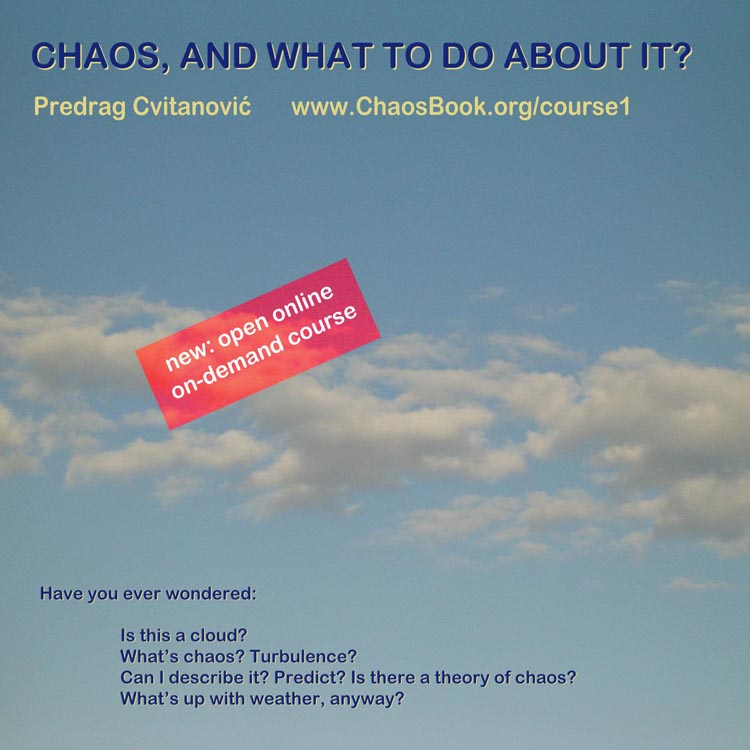
\includegraphics[width=0.65\textwidth]{posterCB2cover}
\end{center}
\vfill
student raves : \\
...$10^6$ times harder than any other online course...
\end{frame}



\end{document}
